\chapter{HASIL DAN PEMBAHASAN}
\label{chap:hasil_dan_pembahasan}

\section{Gambaran Umum Pelaksanaan Pengujian}
\label{sec:gambaran_pengujian}
Seluruh pengujian pada penelitian ini dilaksanakan pada lingkungan simulasi Gazebo~11 yang terintegrasi dengan ROS Noetic sesuai arsitektur sistem yang telah dijelaskan pada Bab~III. Proses eksperimen dilakukan untuk mengevaluasi pengaruh integrasi kamera termal, fusi trav\-ersability LiDAR--termal, serta pengendali fuzzy Mamdani terhadap performa navigasi robot bergerak pada berbagai kondisi lingkungan. Fokus evaluasi diarahkan pada kemampuan sistem dalam mempertahankan margin keselamatan navigasi, mendeteksi obstacle pada area \textit{blind-spot} LiDAR, serta menjaga efisiensi pergerakan robot menuju tujuan.

Pelaksanaan eksperimen mengikuti prosedur pengujian yang telah dijelaskan pada Subbab~\ref{sec:eksperimen}. Setiap skenario dijalankan sebanyak sepuluh kali percobaan independen ($n = 10$) menggunakan konfigurasi awal yang identik. Dengan delapan skenario pengujian yang terdiri atas empat skenario \textit{baseline} dan empat skenario \textit{fuzzy}, total diperoleh 80 \textit{trial} yang digunakan sebagai dasar analisis pada bab ini. Seluruh data eksperimen direkam secara otomatis menggunakan node \texttt{experiment\_logger.py} dan disimpan ke dalam direktori \texttt{experiment\_data} untuk selanjutnya diproses pada tahap analisis statistik.

Kedelapan skenario pengujian disusun dalam empat pasangan perbandingan yang mewakili kondisi lingkungan yang sama namun menggunakan konfigurasi kendali yang berbeda. Pas\-angan S1 dan S5 merepresentasikan lingkungan terbuka tanpa obstacle. Pasangan S2 dan S6 merepresentasikan lingkungan dengan satu obstacle manusia statis. Pasangan S3 dan S7 merepresentasikan lingkungan dengan beberapa obstacle statis yang mencakup keberadaan obstacle berprofil rendah berupa kucing pada area \textit{blind-spot} LiDAR. Sementara itu, pasangan S4 dan S8 merepresentasikan lingkungan dengan obstacle dinamis yang bergerak melintasi jalur robot serta keberadaan obstacle kucing pada area \textit{blind-spot}. Konfigurasi tersebut dipilih untuk mengevaluasi performa sistem pada tingkat kompleksitas lingkungan yang semakin meningkat.

Pada seluruh skenario, konfigurasi sensor yang digunakan tetap sama, yaitu sensor LiDAR 2D dan kamera termal yang aktif secara bersamaan. Kedua sensor diproses melalui \textit{pipeline} yang identik sehingga menghasilkan informasi traversability berbasis LiDAR, traversability berbasis termal, serta traversability efektif hasil fusi sensor. Informasi tersebut kemudian digunakan oleh APFPlanner untuk menghasilkan perintah navigasi robot. Perbedaan utama antara kelompok \textit{baseline} (S1--S4) dan kelompok \textit{fuzzy} (S5--S8) terletak pada penggunaan pengendali fuzzy Mamdani sebagai mekanisme adaptasi parameter navigasi. Pada konfigurasi \textit{baseline}, parameter APF menggunakan nilai tetap, sedangkan pada konfigurasi \textit{fuzzy}, parameter \textit{speed scale} dan \textit{repulsive gain} disesuaikan secara adaptif berdasarkan nilai jarak obstacle terdekat dan traversability efektif sebagaimana dijelaskan pada Subbab~\ref{sec:fuzzy_Aapf}.

Data primer yang diperoleh dari setiap \textit{trial} meliputi status keberhasilan navigasi, jumlah tabrakan, nilai minimum clearance, waktu tempuh, panjang lintasan, kecepatan linear rata-rata, dan kecepatan angular rata-rata. Seluruh data tersebut direkam secara \textit{real-time} selama eksperimen berlangsung dan kemudian diproses menggunakan skrip analisis untuk menghasilkan statistik deskriptif serta hasil uji inferensial. Analisis statistik dilakukan menggunakan uji Mann--Whitney U dan \textit{rank-biserial correlation} sesuai metode yang telah dijelaskan pada Subbab~\ref{sec:evaluasi}.

Penyajian hasil pada bab ini mengikuti urutan tujuan evaluasi yang telah ditetapkan pada Subbab~\ref{sec:evaluasi}. Pembahasan diawali dengan penyajian hasil deskriptif pada masing-masing skenario untuk memberikan gambaran umum performa sistem. Selanjutnya dilakukan evaluasi tingkat keberhasilan navigasi dan ketiadaan tabrakan pada seluruh skenario pengujian. Analisis kemudian difokuskan pada \textit{minimum clearance} sebagai metrik utama yang digunakan untuk menilai peningkatan keselamatan navigasi akibat integrasi kamera termal dan pengendali fuzzy. Setelah itu dibahas \textit{trade-off} yang muncul terhadap efisiensi navigasi melalui analisis waktu tempuh dan panjang lintasan, serta kehalusan pergerakan robot berdasarkan karakteristik kecepatan angular. Untuk memperkuat temuan kuantitatif, beberapa visualisasi trajektori robot juga disajikan pada skenario yang memiliki tingkat kompleksitas tertinggi. Seluruh hasil pengujian kemudian dirangkum dan dibahas secara terintegrasi untuk menjawab tujuan penelitian yang telah dirumuskan pada Bab~I.


\section{Hasil Deskriptif Pengujian}
\label{sec:hasil_deskriptif}
Subbab ini menyajikan gambaran umum hasil eksperimen yang diperoleh dari seluruh skenario pengujian sebelum dilakukan analisis statistik yang lebih mendalam pada subbab berikutnya. Penyajian secara deskriptif bertujuan untuk memberikan pemahaman awal mengenai karakteristik performa sistem navigasi pada konfigurasi \textit{baseline} maupun konfigurasi \textit{fuzzy}. Fokus pembahasan diarahkan pada tren umum yang muncul selama pengujian, sedangkan evaluasi signifikansi statistik dibahas pada Subbab~4.7.

Sebanyak delapan skenario pengujian telah dilaksanakan sesuai prosedur yang dijelaskan pada Bab~III. Setiap skenario dijalankan sebanyak sepuluh kali percobaan independen sehingga diperoleh total 80 \textit{trial}. Data hasil eksperimen kemudian diolah untuk memperoleh metrik evaluasi yang meliputi tingkat keberhasilan navigasi, \textit{collision-free rate}, \textit{minimum clearance}, waktu navigasi, panjang lintasan, kecepatan linear rata-rata, dan kecepatan angular rata-rata.

\subsection{Ringkasan Hasil Seluruh Skenario}

Tabel~\ref{tab:ringkasan_hasil_deskriptif} menyajikan ringkasan hasil pengujian pada seluruh skenario.

\begin{table}[H]
\centering
\caption{Ringkasan hasil deskriptif seluruh skenario pengujian.}
\label{tab:ringkasan_hasil_deskriptif}
\begin{tabular}{cccccc}
\toprule
Skenario &
$SR$ (\%) &
$CFR$ (\%) &
$c_{min}$ (m) &
$t_{nav}$ (s) &
$L$ (m) \\
\midrule
S1 & 100 & 100 & 0.000 & 25.50 & 11.26 \\
S2 & 100 & 100 & 0.430 & 29.72 & 12.03 \\
S3 & 65  & 65  & 0.035 & 29.51 & 12.15 \\
S4 & 0   & 0   & -0.164 & 33.47 & 11.79 \\
S5 & 100 & 100 & 0.000 & 31.04 & 11.25 \\
S6 & 100 & 100 & 0.437 & 34.35 & 11.94 \\
S7 & 100 & 100 & 0.182 & 48.26 & 12.87 \\
S8 & 100 & 100 & 0.317 & 49.97 & 12.41 \\
\bottomrule
\end{tabular}
\end{table}

Secara umum, seluruh konfigurasi mampu menyelesaikan tugas navigasi dengan baik pada lingkungan yang relatif sederhana. Hal ini ditunjukkan oleh tingkat keberhasilan sebesar 100\% pada skenario S1, S2, S5, dan S6. Pada kondisi tersebut, baik konfigurasi \textit{baseline} maupun konfigurasi \textit{fuzzy} mampu mencapai tujuan tanpa mengalami tabrakan.

Perbedaan performa mulai terlihat ketika kompleksitas lingkungan meningkat. Pada skenario S3 yang melibatkan beberapa obstacle statis serta obstacle berprofil rendah pada area \textit{blind-spot} LiDAR, konfigurasi \textit{baseline} hanya mencapai tingkat keberhasilan sebesar 65\%. Kondisi yang lebih menantang ditunjukkan oleh skenario S4, di mana seluruh percobaan gagal mencapai tujuan tanpa tabrakan. Nilai \textit{minimum clearance} yang negatif pada S4 mengindikasi\-kan bahwa robot mengalami kontak langsung dengan obstacle selama navigasi.

Sebaliknya, seluruh percobaan pada konfigurasi fuzzy (S5--S8) berhasil mencapai tujuan dengan tingkat keberhasilan dan \textit{collision-free rate} sebesar 100\%. Peningkatan tersebut paling terlihat pada pasangan S3--S7 dan S4--S8, yaitu ketika robot harus beroperasi pada lingkungan yang mengandung obstacle berprofil rendah maupun obstacle dinamis.

\subsection{Perbandingan Kelompok Baseline dan Fuzzy}

Perbandingan antara kelompok \textit{baseline} dan \textit{fuzzy} dilakukan menggunakan empat pasangan skenario yang memiliki kondisi lingkungan identik, yaitu S1--S5, S2--S6, S3--S7, dan S4--S8.

Pada pasangan S1--S5 dan S2--S6, kedua konfigurasi menghasilkan performa yang relatif serupa. Seluruh percobaan berhasil mencapai tujuan dan tidak ditemukan tabrakan. Perbedaan utama hanya terlihat pada waktu navigasi yang sedikit lebih tinggi pada konfigurasi fuzzy akibat mekanisme penyesuaian kecepatan yang lebih konservatif.

Perbedaan yang lebih signifikan muncul pada pasangan S3--S7 dan S4--S8. Pada kedua pasangan tersebut, konfigurasi fuzzy menunjukkan peningkatan tingkat keberhasilan yang disertai dengan peningkatan \textit{minimum clearance}. Nilai clearance rata-rata meningkat dari 0,035 m pada S3 menjadi 0,182 m pada S7, serta dari -0,164 m pada S4 menjadi 0,317 m pada S8. Temuan ini menunjukkan bahwa robot mampu mempertahankan jarak aman yang lebih besar terhadap obstacle ketika mekanisme adaptasi fuzzy diaktifkan.

Di sisi lain, peningkatan margin keselamatan tersebut diikuti oleh kenaikan waktu navigasi. Rata-rata waktu tempuh pada S7 dan S8 lebih tinggi dibandingkan pasangan \textit{baseline}-nya, yang mengindikasikan adanya \textit{trade-off} antara keselamatan dan efisiensi navigasi.

\subsection{Observasi Kualitatif Perilaku Navigasi}

Selain metrik kuantitatif, perilaku navigasi robot juga diamati melalui visualisasi trajektori dan pengamatan langsung selama simulasi berlangsung.

Pada konfigurasi \textit{baseline}, robot cenderung mempertahankan kecepatan yang relatif konstan selama bergerak menuju tujuan. Strategi tersebut menghasilkan waktu tempuh yang lebih singkat, namun pada beberapa kondisi menyebabkan robot melakukan manuver penghindaran dengan jarak yang sangat dekat terhadap obstacle. Fenomena ini terutama terlihat pada skenario yang melibatkan obstacle berprofil rendah dan obstacle dinamis.

Sebaliknya, konfigurasi fuzzy menunjukkan perilaku yang lebih adaptif terhadap perubahan kondisi lingkungan. Ketika obstacle terdeteksi pada jarak yang dekat atau traversability lingkungan menurun, robot secara bertahap mengurangi kecepatan dan meningkatkan respons penghindaran obstacle. Akibatnya, robot mampu mempertahankan margin keselamatan yang lebih besar dan mengurangi risiko tabrakan.

Secara keseluruhan, hasil deskriptif menunjukkan bahwa integrasi kamera termal, fusi traversability, dan pengendali fuzzy memberikan kontribusi positif terhadap keamanan navigasi robot, khususnya pada lingkungan yang mengandung obstacle berprofil rendah maupun obstacle dinamis. Temuan awal ini akan dianalisis lebih lanjut secara kuantitatif pada subbab-subbab berikutnya menggunakan metrik evaluasi dan metode statistik yang telah dijelaskan pada Bab~III.

\section{Tingkat Keberhasilan Navigasi dan Collision-Free Rate}
\label{sec:success_rate}
Tingkat keberhasilan navigasi (\textit{Success Rate}) dan \textit{Collision-Free Rate} (CFR) digunakan sebagai indikator awal untuk mengevaluasi kemampuan sistem dalam mencapai tujuan navigasi tanpa mengalami tabrakan. Kedua metrik ini memberikan gambaran mengenai reliabilitas sistem pada berbagai tingkat kompleksitas lingkungan sebelum dilakukan analisis yang lebih rinci terhadap margin keselamatan, efisiensi navigasi, dan karakteristik pergerakan robot.

\subsection{Success Rate}

Success Rate menunjukkan persentase percobaan yang berhasil mencapai tujuan navigasi dalam batas waktu yang ditentukan tanpa mengalami kegagalan navigasi. Nilai Success Rate pada seluruh skenario ditunjukkan pada Tabel~\ref{tab:success_rate}.

\begin{table}[H]
\centering
\caption{Perbandingan Success Rate pada seluruh skenario pengujian.}
\label{tab:success_rate}
\begin{tabular}{ccc}
\toprule
Skenario & Konfigurasi & Success Rate (\%) \\
\midrule
S1 & Baseline & 100 \\
S2 & Baseline & 100 \\
S3 & Baseline & 65 \\
S4 & Baseline & 0 \\
S5 & Fuzzy & 100 \\
S6 & Fuzzy & 100 \\
S7 & Fuzzy & 100 \\
S8 & Fuzzy & 100 \\
\bottomrule
\end{tabular}
\end{table}

\begin{figure}[H]
\centering
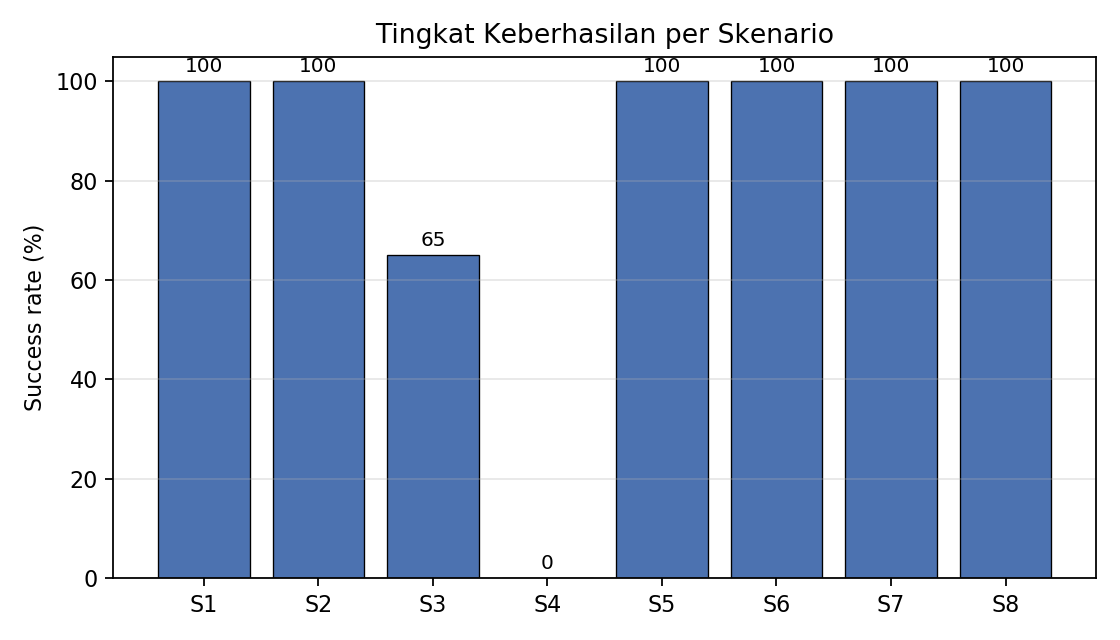
\includegraphics[width=0.6\textwidth]{gambar/4.2_fig_success_rate.png}
\caption{Perbandingan Success Rate pada seluruh skenario pengujian.}
\label{fig:success_rate}
\end{figure}

Hasil pengujian menunjukkan bahwa seluruh percobaan pada S1, S2, S5, dan S6 berhasil mencapai tujuan navigasi. Kondisi ini menunjukkan bahwa baik konfigurasi baseline maupun konfigurasi fuzzy mampu menyelesaikan tugas navigasi secara konsisten pada lingkungan terbuka maupun lingkungan dengan satu obstacle manusia statis.

Perbedaan performa mulai terlihat pada skenario yang memiliki tingkat kompleksitas lebih tinggi. Pada S3, konfigurasi baseline hanya berhasil menyelesaikan 65\% percobaan, sedangkan konfigurasi fuzzy pada S7 mencapai tingkat keberhasilan sebesar 100\%. Peningkatan yang lebih signifikan terlihat pada pasangan S4 dan S8. Seluruh percobaan pada S4 gagal mencapai tujuan sehingga menghasilkan Success Rate sebesar 0\%, sedangkan seluruh percobaan pada S8 berhasil mencapai tujuan dengan Success Rate sebesar 100\%.

Hasil tersebut menunjukkan bahwa metode yang diusulkan memberikan peningkatan reliabilitas navigasi terutama pada lingkungan yang mengandung obstacle berprofil rendah pada area \textit{blind-spot} LiDAR dan obstacle dinamis. Pada kondisi tersebut, informasi tambahan yang diperoleh dari kamera termal memungkinkan sistem mengenali obstacle yang tidak sepenuhnya terdeteksi oleh LiDAR, sementara mekanisme fuzzy membantu robot menyesuaikan perilaku navigasi secara lebih adaptif.

\subsection{Collision-Free Rate}

Selain tingkat keberhasilan navigasi, keamanan sistem juga dievaluasi menggunakan Coll\-ision-Free Rate (CFR). Metrik ini menunjukkan persentase percobaan yang dapat diselesaikan tanpa terjadinya kontak fisik antara robot dan obstacle. Hasil pengujian CFR ditunjukkan pada Tabel\\~\ref{tab:cfr}.

\begin{table}[H]
\centering
\caption{Perbandingan Collision-Free Rate pada seluruh skenario pengujian.}
\label{tab:cfr}
\begin{tabular}{ccc}
\toprule
Skenario & Konfigurasi & CFR (\%) \\
\midrule
S1 & Baseline & 100 \\
S2 & Baseline & 100 \\
S3 & Baseline & 65 \\
S4 & Baseline & 0 \\
S5 & Fuzzy & 100 \\
S6 & Fuzzy & 100 \\
S7 & Fuzzy & 100 \\
S8 & Fuzzy & 100 \\
\bottomrule
\end{tabular}
\end{table}

Nilai CFR menunjukkan pola yang serupa dengan Success Rate. Seluruh percobaan pada S1, S2, S5, dan S6 berhasil diselesaikan tanpa tabrakan. Namun demikian, ketika robot beroperasi pada lingkungan yang lebih kompleks, konfigurasi baseline mengalami penurunan performa yang cukup signifikan.

Pada S3, hanya 65\% percobaan yang dapat diselesaikan tanpa tabrakan. Kondisi yang lebih ekstrem terlihat pada S4, di mana seluruh percobaan mengalami tabrakan sehingga menghasilkan CFR sebesar 0\%. Hasil tersebut menunjukkan bahwa keberadaan obstacle berprofil rendah dan obstacle dinamis menjadi tantangan yang sulit diatasi oleh konfigurasi baseline.

Sebaliknya, konfigurasi fuzzy mempertahankan CFR sebesar 100\% pada seluruh skenario pengujian. Peningkatan ini mengindikasikan bahwa integrasi kamera termal dan mekanisme adaptasi fuzzy mampu meningkatkan kemampuan sistem dalam menghindari obstacle secara konsisten. Dengan memanfaatkan informasi traversability hasil fusi sensor, robot dapat mempertahankan jarak aman yang lebih besar terhadap obstacle sehingga risiko tabrakan dapat diminimalkan.

Temuan pada subbab ini menunjukkan bahwa perbedaan performa antara konfigurasi baseline dan fuzzy relatif kecil pada lingkungan yang sederhana, namun menjadi sangat signifikan ketika robot beroperasi pada lingkungan yang mengandung obstacle berprofil rendah maupun obstacle dinamis. Untuk memahami peningkatan keselamatan navigasi secara lebih rinci, analisis pada subbab berikutnya difokuskan pada evaluasi \textit{minimum clearance} sebagai metrik utama penelitian ini.

\section{Analisis Minimum Clearance}
\label{sec:minimum_clearance}
Sebagaimana dijelaskan pada Subbab~3.9, \textit{minimum clearance} dipilih sebagai metrik uta\-ma dalam penelitian ini karena secara langsung merepresentasikan margin keselamatan yang dipertahankan robot terhadap obstacle selama proses navigasi berlangsung. Berbeda dengan \textit{success rate} yang hanya menunjukkan hasil akhir navigasi, \textit{minimum clearance} mampu mengg\-ambarkan tingkat risiko kolisi yang dialami robot sepanjang lintasan yang ditempuh.

Pada penelitian ini, nilai \textit{minimum clearance} dihitung sebagai jarak bebas minimum antara batas luar robot dan obstacle terdekat yang teramati selama satu percobaan. Semakin besar nilai \textit{minimum clearance}, semakin besar pula margin keselamatan yang dipertahankan robot ketika bergerak menuju tujuan.

\subsection{Perbandingan Minimum Clearance}

Nilai rata-rata \textit{minimum clearance} pada seluruh skenario ditunjukkan pada Tabel~\ref{tab:min_clearance}.

\begin{table}[H]
\centering
\caption{Perbandingan nilai minimum clearance pada seluruh skenario pengujian.}
\label{tab:min_clearance}
\begin{tabular}{ccc}
\toprule
Skenario & Konfigurasi & Minimum Clearance (m) \\
\midrule
S1 & Baseline & 0.0000 \\
S2 & Baseline & 0.4301 \\
S3 & Baseline & 0.0346 \\
S4 & Baseline & -0.1635 \\
S5 & Fuzzy & 0.0000 \\
S6 & Fuzzy & 0.4370 \\
S7 & Fuzzy & 0.1825 \\
S8 & Fuzzy & 0.3167 \\
\bottomrule
\end{tabular}
\end{table}

\begin{figure}[H]
\centering
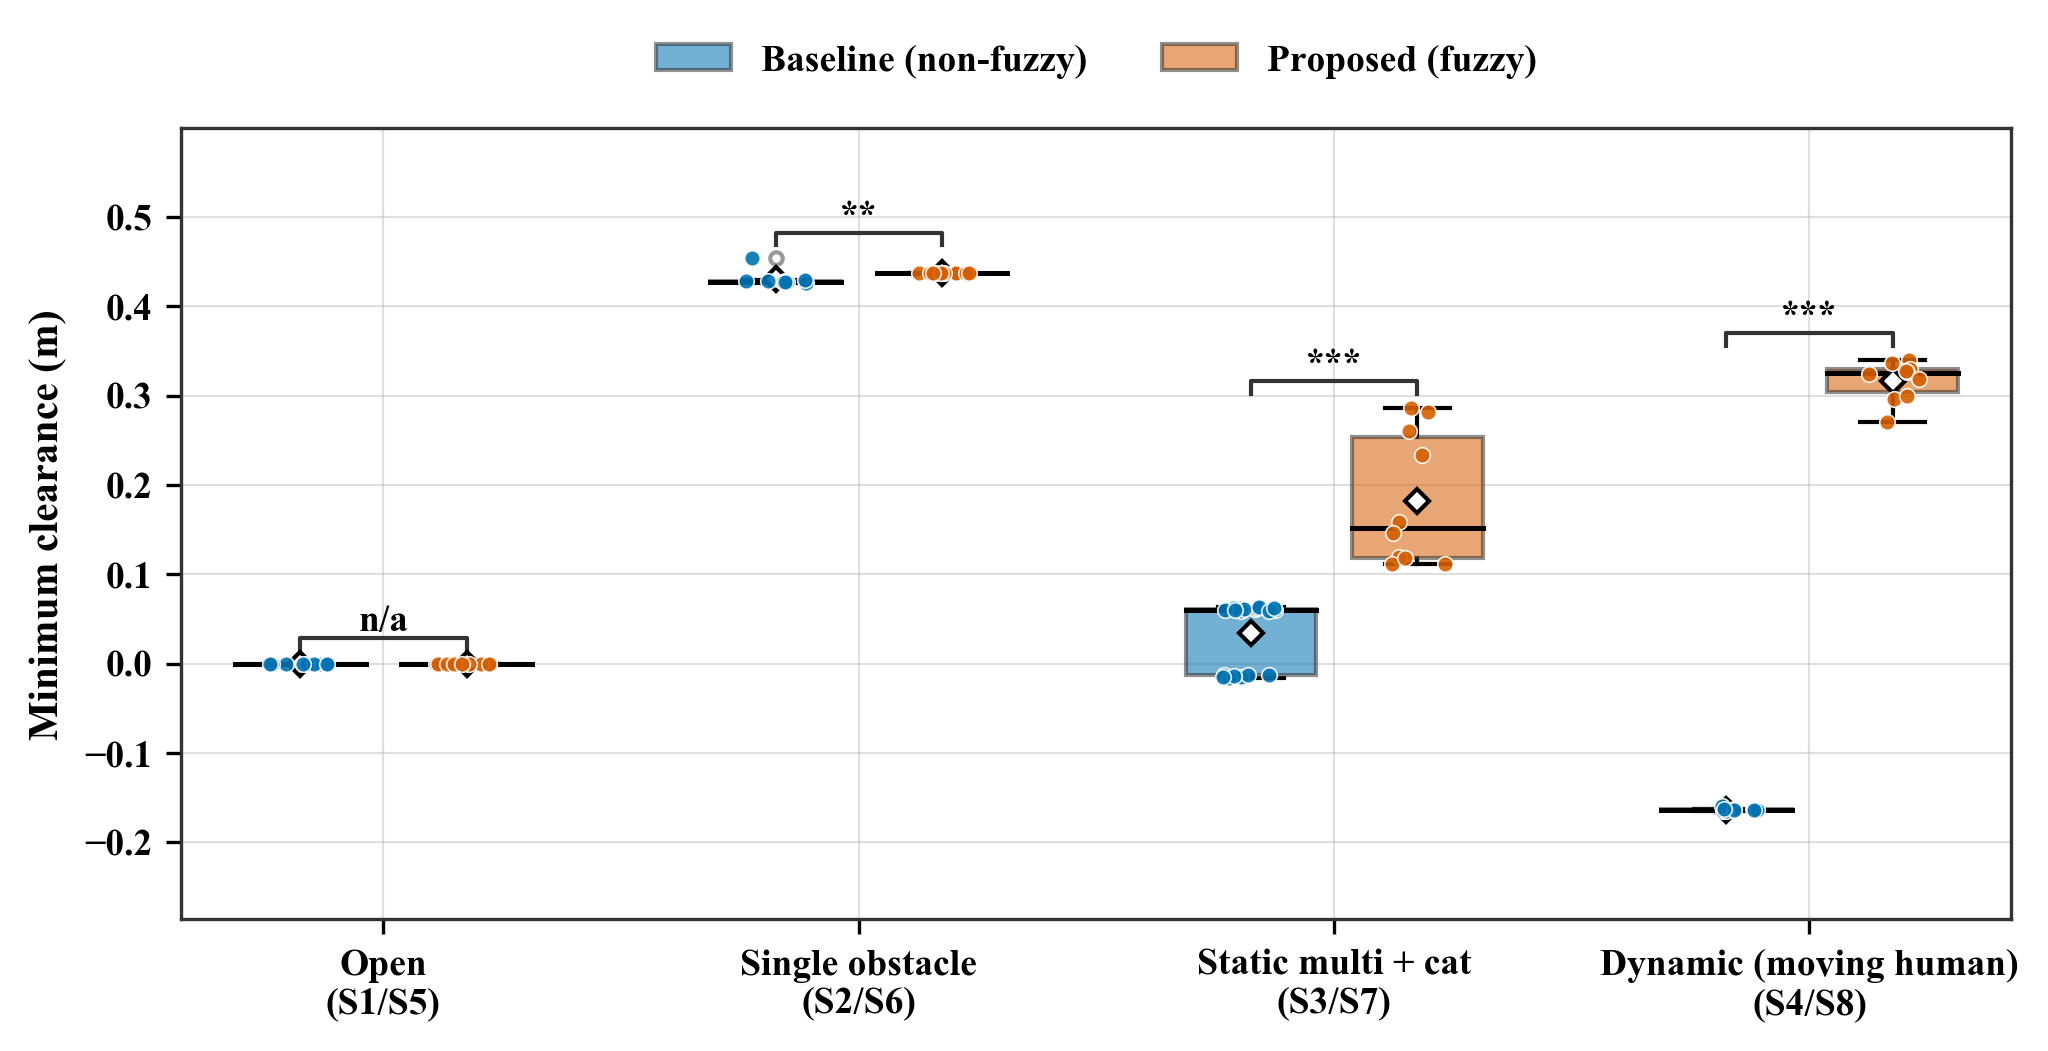
\includegraphics[width=0.7\textwidth]{gambar/4.4_fig_clearance_mean.png}
\caption{Perbandingan rata-rata minimum clearance pada seluruh skenario pengujian.}
\label{fig:mean_clearance}
\end{figure}

Secara umum, konfigurasi fuzzy menghasilkan nilai \textit{minimum clearance} yang lebih tinggi dibandingkan konfigurasi baseline pada seluruh pasangan skenario yang mengandung obstacle. Perbedaan tersebut relatif kecil pada lingkungan sederhana, namun meningkat secara signifikan ketika robot beroperasi pada lingkungan yang mengandung obstacle berprofil rendah dan obstacle dinamis.

Pada pasangan S2--S6, nilai \textit{minimum clearance} meningkat dari 0,4301~m menjadi 0,4370\\~m. Peningkatan ini relatif kecil karena kedua konfigurasi sama-sama mampu mendeteksi obstacle manusia yang berada dalam jangkauan observasi LiDAR. Oleh karena itu, kontribusi kamera termal dan mekanisme fuzzy belum terlihat secara dominan pada skenario ini.

Perbedaan yang lebih jelas terlihat pada pasangan S3--S7. Pada konfigurasi baseline, robot hanya mampu mempertahankan \textit{minimum clearance} sebesar 0,0346~m. Nilai tersebut menunjukkan bahwa robot bergerak sangat dekat dengan obstacle selama navigasi berlangsung. Setelah mekanisme fuzzy diaktifkan, nilai \textit{minimum clearance} meningkat menjadi 0,1825~m atau lebih dari lima kali lipat dibandingkan konfigurasi baseline.

Peningkatan yang paling signifikan terjadi pada pasangan S4--S8. Pada konfigurasi baseline, nilai \textit{minimum clearance} bernilai negatif sebesar -0,1635~m. Nilai negatif menunjukkan bahwa robot mengalami kontak dengan obstacle selama navigasi. Sebaliknya, konfigurasi fuzzy mampu mempertahankan \textit{minimum clearance} positif sebesar 0,3167~m sehingga seluruh percobaan dapat diselesaikan tanpa tabrakan. Hasil ini menunjukkan bahwa metode yang diusulkan mampu meningkatkan margin keselamatan secara substansial pada lingkungan dengan tingkat kompleksitas tinggi.

\subsection{Distribusi Minimum Clearance}

Untuk memperoleh gambaran yang lebih komprehensif mengenai penyebaran data, distribusi \textit{minimum clearance} pada setiap pasangan skenario divisualisasikan menggunakan boxplot sebagaimana ditunjukkan pada Gambar~\ref{fig:boxplot_clearance}.

\begin{figure}[H]
\centering
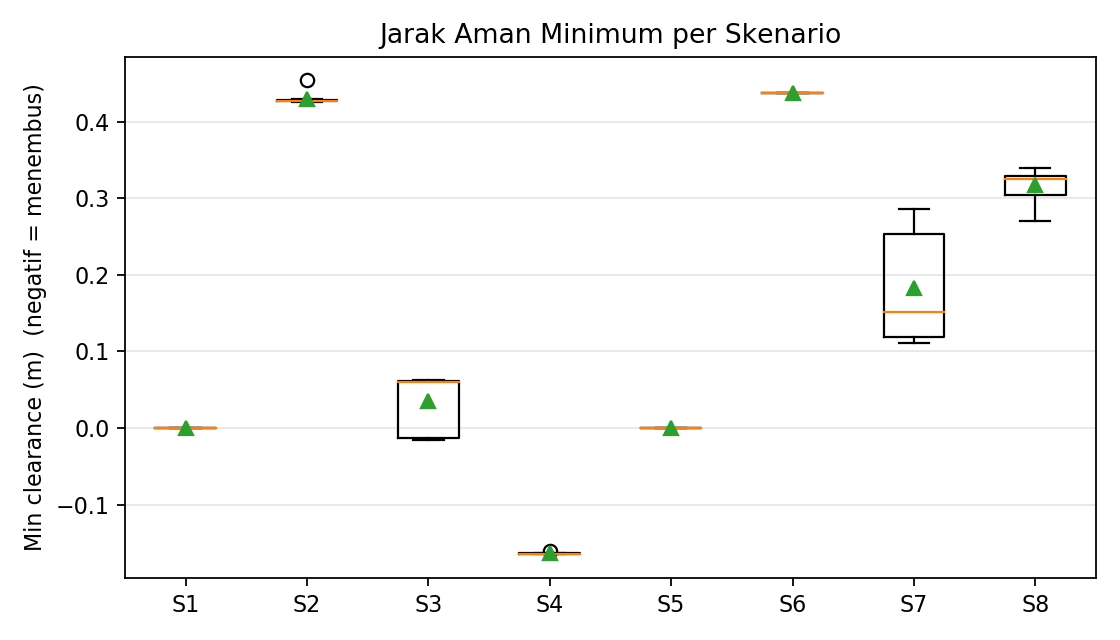
\includegraphics[width=0.9\textwidth]{gambar/4.4_fig_clearance_box.png}
\caption{Distribusi minimum clearance pada seluruh pasangan skenario pengujian.}
\label{fig:boxplot_clearance}
\end{figure}

Distribusi data pada Gambar~\ref{fig:boxplot_clearance} menunjukkan bahwa konfigurasi fuzzy tidak hanya meni\-ngkatkan nilai rata-rata \textit{minimum clearance}, tetapi juga menggeser keseluruhan distribusi data menuju nilai clearance yang lebih tinggi. Pergeseran tersebut terlihat paling jelas pada pasangan S3--S7 dan S4--S8 yang merepresentasikan lingkungan dengan tingkat kompleksitas tinggi.

Pada pasangan S3--S7, sebagian besar percobaan pada konfigurasi baseline menghasilkan clearance yang sangat kecil sehingga robot bergerak dalam jarak yang sangat dekat terhadap obstacle. Setelah mekanisme fuzzy diaktifkan, distribusi data bergeser ke arah nilai yang lebih besar dan menunjukkan bahwa robot secara konsisten mempertahankan jarak aman selama navigasi berlangsung.

Fenomena yang lebih menonjol terlihat pada pasangan S4--S8. Distribusi data pada S4 menunjukkan adanya sejumlah percobaan dengan nilai clearance negatif yang mengindikasikan terjadinya tabrakan. Sebaliknya, seluruh distribusi pada S8 berada pada daerah clearance positif dengan median yang jauh lebih tinggi. Hasil tersebut menunjukkan bahwa metode yang diusulkan tidak hanya meningkatkan rata-rata clearance, tetapi juga menghilangkan kejadian tabrakan yang sebelumnya muncul pada konfigurasi baseline.

\subsection{Analisis Statistik Minimum Clearance}

Untuk mengevaluasi apakah perbedaan yang diamati bersifat signifikan secara statistik, dilakukan uji Mann--Whitney U terhadap setiap pasangan skenario yang memiliki kondisi lingku\-ngan identik. Hasil pengujian ditunjukkan pada Tabel~\ref{tab:mw_clearance}.

\begin{table}[H]
\centering
\caption{Hasil uji Mann--Whitney U untuk minimum clearance.}
\label{tab:mw_clearance}
\begin{tabular}{cccc}
\toprule
Pasangan &
$p$-value &
Effect Size ($r$) &
Interpretasi \\
\midrule
S1--S5 & n/a & n/a & Tidak berbeda \\
S2--S6 & 0.0013 & 0.80 & Besar \\
S3--S7 & $<0.001$ & 1.00 & Sangat besar \\
S4--S8 & 0.0002 & 1.00 & Sangat besar \\
\bottomrule
\end{tabular}
\end{table}
Hasil uji Mann--Whitney U menunjukkan bahwa peningkatan
\textit{minimum clearance} pada konfigurasi fuzzy bersifat
signifikan secara statistik pada seluruh skenario yang
mengandung obstacle. Pada pasangan S2--S6 diperoleh
$p=0.0013$ dengan \textit{effect size} sebesar $r=0.80$,
yang termasuk kategori besar. Meskipun peningkatan
clearance pada skenario ini relatif kecil secara absolut,
hasil tersebut menunjukkan bahwa konfigurasi fuzzy secara
konsisten mempertahankan jarak aman yang lebih tinggi
dibandingkan konfigurasi baseline.

Perbedaan yang lebih kuat terlihat pada pasangan S3--S7
dan S4--S8. Pada kedua pasangan tersebut diperoleh
nilai $p<0.001$ dengan \textit{effect size} sebesar
$r=1.00$, yang menunjukkan perbedaan sangat besar antara
kedua kelompok. Hasil ini mengindikasikan bahwa seluruh
distribusi data pada konfigurasi fuzzy bergeser menuju
nilai clearance yang lebih tinggi dibandingkan konfigurasi
baseline.

Temuan tersebut memperkuat hasil deskriptif yang telah
ditunjukkan pada subbab sebelumnya. Pada lingkungan yang
mengandung obstacle berprofil rendah dan obstacle dinamis,
integrasi kamera termal memungkinkan sistem mendeteksi
hambatan yang tidak sepenuhnya teramati oleh LiDAR 2D,
sementara pengendali fuzzy menyesuaikan parameter
\textit{speed scale} dan \textit{repulsive gain}
secara adaptif ketika tingkat traversability menurun.
Kombinasi kedua mekanisme tersebut menghasilkan peningkatan
margin keselamatan yang signifikan dan konsisten pada
berbagai kondisi pengujian.

Berdasarkan hasil tersebut, hipotesis H1 yang menyatakan
bahwa metode usulan menghasilkan nilai \textit{minimum clearance}
yang lebih tinggi dibandingkan konfigurasi baseline dapat
diterima.

\section{Analisis Efisiensi Navigasi}
\label{sec:efisiensi_navigasi}
Selain meningkatkan keselamatan navigasi, metode yang diusulkan juga perlu dievaluasi dari sisi efisiensi pergerakan robot. Pada sistem navigasi robot bergerak, peningkatan margin keselamatan sering kali diikuti oleh konsekuensi berupa penambahan waktu tempuh atau perubahan karakteristik lintasan karena robot mempertahankan jarak yang lebih besar terhadap obstacle. Oleh karena itu, efisiensi navigasi pada penelitian ini dievaluasi menggunakan dua metrik utama, yaitu waktu tempuh (\textit{traversal time}) dan panjang lintasan (\textit{path length}).

\subsection{Analisis Waktu Tempuh}

Waktu tempuh menunjukkan durasi yang dibutuhkan robot untuk bergerak dari posisi awal menuju titik tujuan. Nilai ini merepresentasikan efisiensi temporal sistem navigasi. Semakin kecil waktu tempuh yang diperlukan, semakin cepat robot menyelesaikan tugas navigasi yang diberikan.

Perbandingan waktu tempuh antara konfigurasi baseline dan fuzzy pada seluruh pasangan skenario ditunjukkan pada Gambar~\ref{fig:traversal_time_compare}.

\begin{figure}[H]
\centering
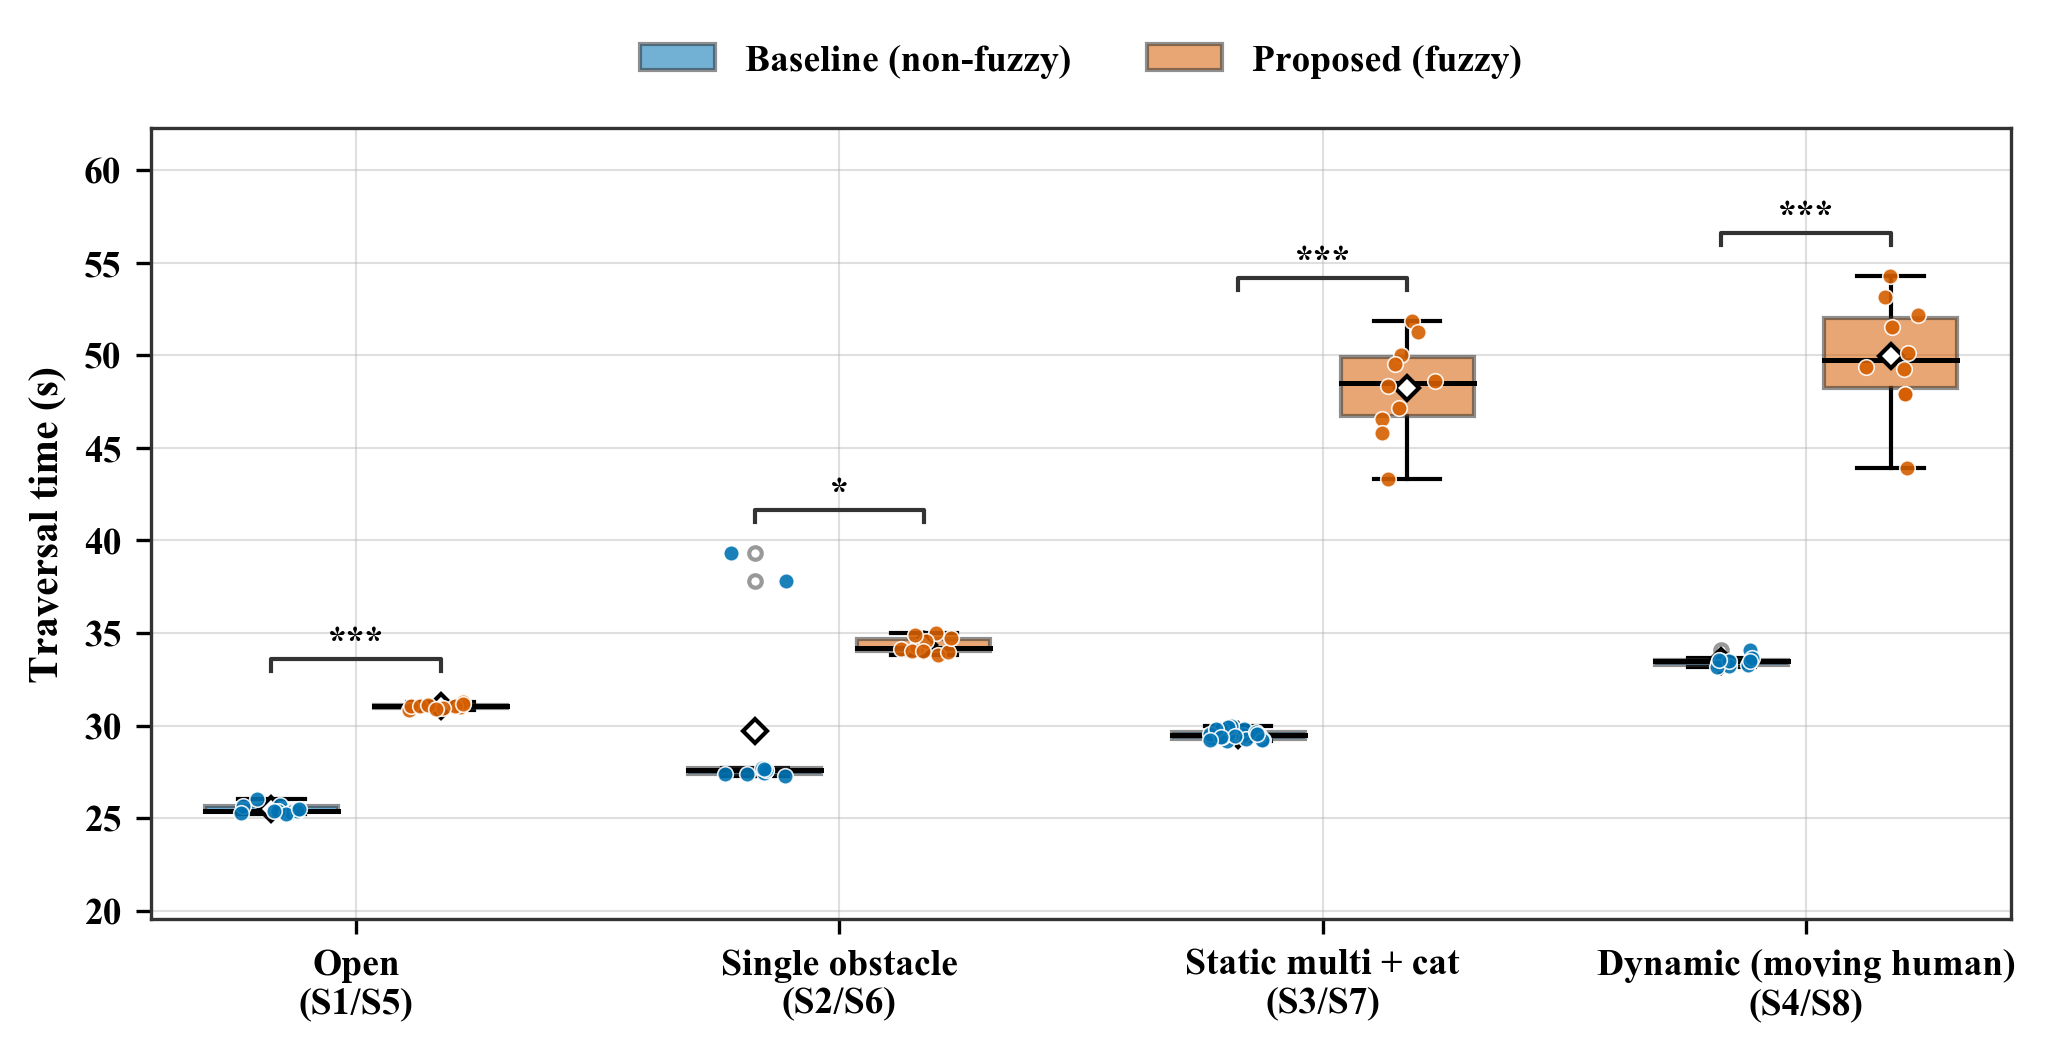
\includegraphics[width=0.6\textwidth]{gambar/fig_time.png}
\caption{Perbandingan waktu tempuh antara konfigurasi baseline dan fuzzy pada seluruh pasangan skenario.}
\label{fig:traversal_time_compare}
\end{figure}

Secara umum terlihat bahwa konfigurasi fuzzy menghasilkan waktu tempuh yang lebih tinggi dibandingkan konfigurasi baseline pada seluruh pasangan skenario. Pada lingkungan terbuka (S1--S5), median waktu tempuh meningkat dari sekitar 25,5 detik menjadi sekitar 31 detik. Peningkatan serupa juga terlihat pada pasangan S2--S6 yang merepresentasikan lingkungan dengan satu obstacle manusia statis.

Perbedaan yang lebih besar muncul pada pasangan S3--S7 dan S4--S8. Pada kedua skenario tersebut, robot dengan konfigurasi fuzzy membutuhkan waktu yang lebih lama untuk mencapai tujuan dibandingkan konfigurasi baseline. Kondisi ini menunjukkan bahwa mekanisme adaptasi fuzzy menyebabkan robot bergerak lebih konservatif ketika mendekati obstacle atau memasuki area dengan nilai traversability yang rendah.

Untuk melihat penyebaran data secara lebih rinci, distribusi waktu tempuh pada setiap skenario divisualisasikan menggunakan boxplot sebagaimana ditunjukkan pada Gambar~\ref{fig:time_boxplot}.

\begin{figure}[H]
\centering
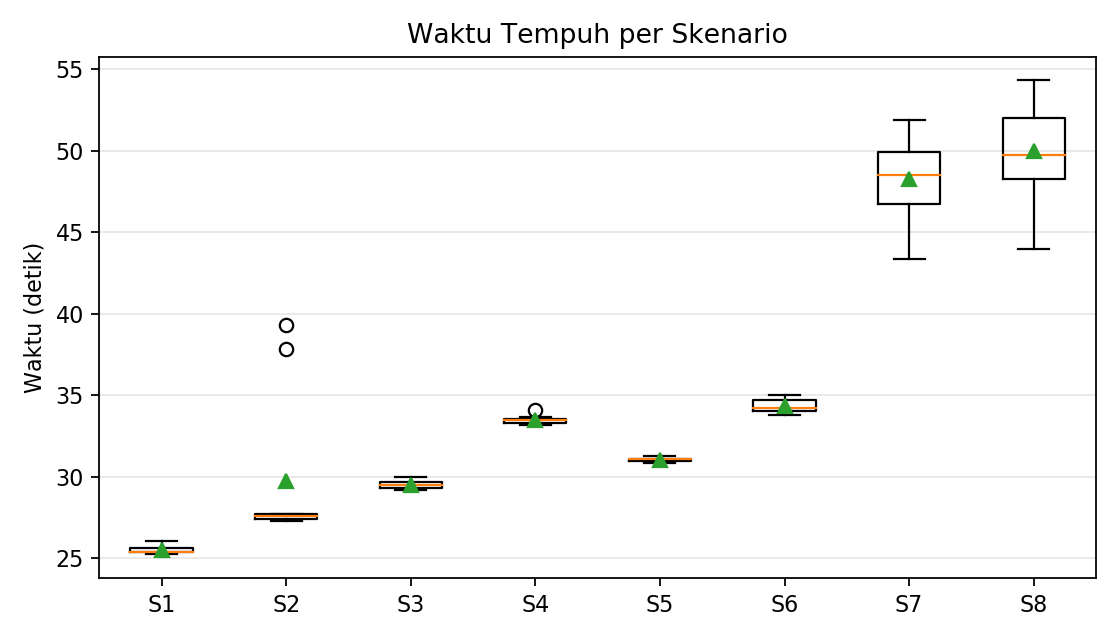
\includegraphics[width=0.6\textwidth]{gambar/fig_time_box.png}
\caption{Distribusi waktu tempuh pada seluruh skenario pengujian.}
\label{fig:time_boxplot}
\end{figure}

Distribusi data menunjukkan bahwa peningkatan waktu tempuh pada konfigurasi fuzzy terjadi secara konsisten pada sebagian besar percobaan. Pada skenario kompleks, khususnya S7 dan S8, peningkatan waktu tempuh sejalan dengan peningkatan \textit{minimum clearance} yang telah dibahas pada Subbab~4.4. Dengan kata lain, robot membutuhkan waktu lebih lama karena mempertahankan jarak aman yang lebih besar terhadap obstacle selama navigasi berlangsung.

Temuan tersebut menunjukkan adanya \textit{trade-off} antara keselamatan dan efisiensi temporal. Mekanisme fuzzy mendorong robot untuk memperlambat pergerakan ketika obstacle berada pada jarak dekat atau ketika nilai traversability lingkungan menurun. Akibatnya, waktu yang dibutuhkan untuk mencapai tujuan meningkat, namun peningkatan tersebut diikuti oleh kenaikan margin keselamatan yang signifikan, terutama pada skenario yang mengandung obstacle berprofil rendah dan obstacle dinamis.

\subsection{Analisis Panjang Lintasan}

Selain waktu tempuh, efisiensi navigasi juga dievaluasi menggunakan panjang lintasan yang ditempuh robot. Metrik ini menggambarkan total jarak yang dilalui robot selama proses navigasi dari titik awal hingga mencapai tujuan.

Distribusi panjang lintasan pada seluruh skenario ditunjukkan pada Gambar~\ref{fig:path_length_boxplot}.

\begin{figure}[H]
\centering
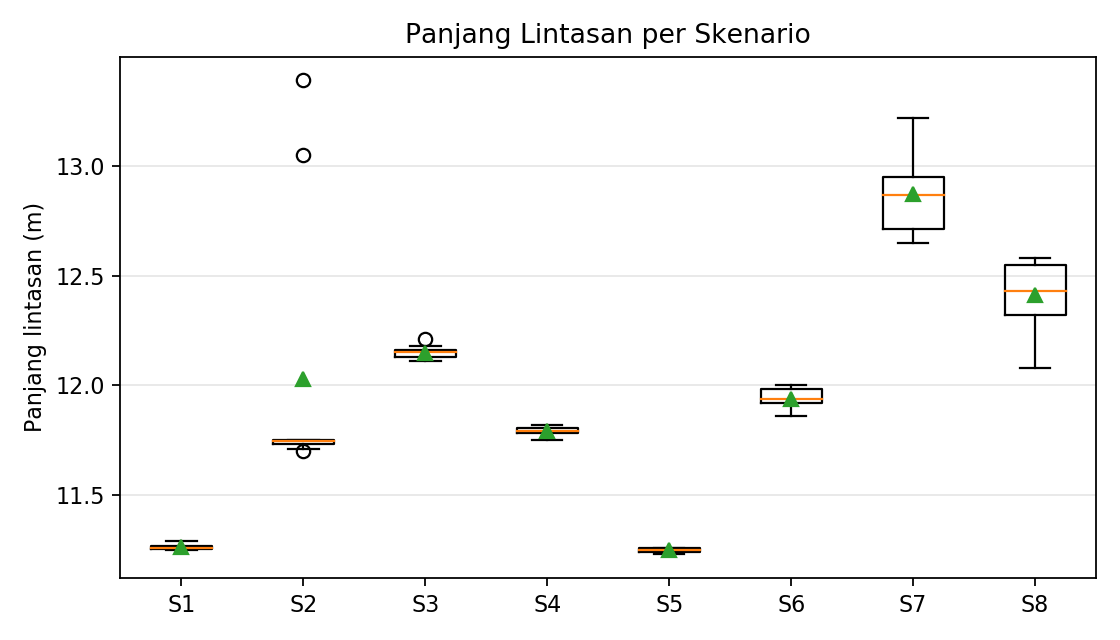
\includegraphics[width=0.6\textwidth]{gambar/fig_path_box.png}
\caption{Distribusi panjang lintasan pada seluruh skenario pengujian.}
\label{fig:path_length_boxplot}
\end{figure}

Hasil pengujian menunjukkan bahwa perbedaan panjang lintasan antara konfigurasi baseline dan fuzzy relatif lebih kecil dibandingkan perbedaan waktu tempuh. Pada lingkungan sederhana, panjang lintasan yang ditempuh kedua konfigurasi cenderung serupa karena robot mengikuti jalur global yang sama dari \textit{NavfnROS}.

Perbedaan mulai terlihat pada lingkungan yang mengandung obstacle berprofil rendah dan obstacle dinamis. Pada konfigurasi fuzzy, robot cenderung mengambil lintasan yang sedikit lebih panjang karena melakukan manuver penghindaran dengan jarak aman yang lebih besar terhadap obstacle. Meskipun demikian, peningkatan panjang lintasan yang terjadi masih berada dalam rentang yang relatif terbatas dibandingkan peningkatan margin keselamatan yang diperoleh.

Hasil ini menunjukkan bahwa peningkatan keselamatan navigasi yang dicapai melalui integrasi kamera termal dan pengendali fuzzy tidak berasal dari perubahan jalur global yang drastis, melainkan dari perubahan perilaku navigasi lokal ketika robot berinteraksi dengan obstacle. Robot tetap mengikuti jalur global yang dihasilkan oleh \textit{NavfnROS}, namun melakukan manuver penghindaran yang lebih konservatif sehingga menghasilkan lintasan yang sedikit lebih panjang.

Dengan mempertimbangkan hasil pada Subbab~4.4, peningkatan panjang lintasan yang terjadi relatif kecil dibandingkan peningkatan margin keselamatan yang diperoleh. Temuan ini mengindikasikan bahwa metode yang diusulkan mampu meningkatkan keselamatan navigasi tanpa menyebabkan degradasi efisiensi lintasan yang signifikan.


\section{Analisis Kehalusan dan Stabilitas Pergerakan}
\label{sec:smoothness}
Selain keselamatan dan efisiensi navigasi, kualitas pergerakan robot juga menjadi aspek penting dalam evaluasi sistem navigasi otonom. Robot yang mampu mencapai tujuan dengan aman belum tentu menghasilkan pergerakan yang stabil apabila selama proses navigasi terjadi perubahan arah yang berlebihan, osilasi, atau manuver yang tidak diperlukan. Oleh karena itu, penelitian ini juga mengevaluasi karakteristik pergerakan robot menggunakan indikator kehalusan (\textit{smoothness}) yang diperoleh dari kecepatan angular selama navigasi berlangsung.

Pada penelitian ini, kehalusan pergerakan dievaluasi menggunakan nilai rata-rata kecepat\-an angular (\textit{average angular velocity}). Nilai ini menggambarkan intensitas perubahan orientasi robot selama bergerak menuju tujuan. Semakin tinggi nilai kecepatan angular, semakin sering robot melakukan manuver belok atau koreksi arah. Sebaliknya, nilai yang lebih rendah menunjukkan pergerakan yang lebih stabil dan halus.

\subsection{Distribusi Kecepatan Angular}

Distribusi kecepatan angular pada seluruh skenario pengujian ditunjukkan pada Gambar~\ref{fig:smoothness_boxplot}.

\begin{figure}[H]
\centering
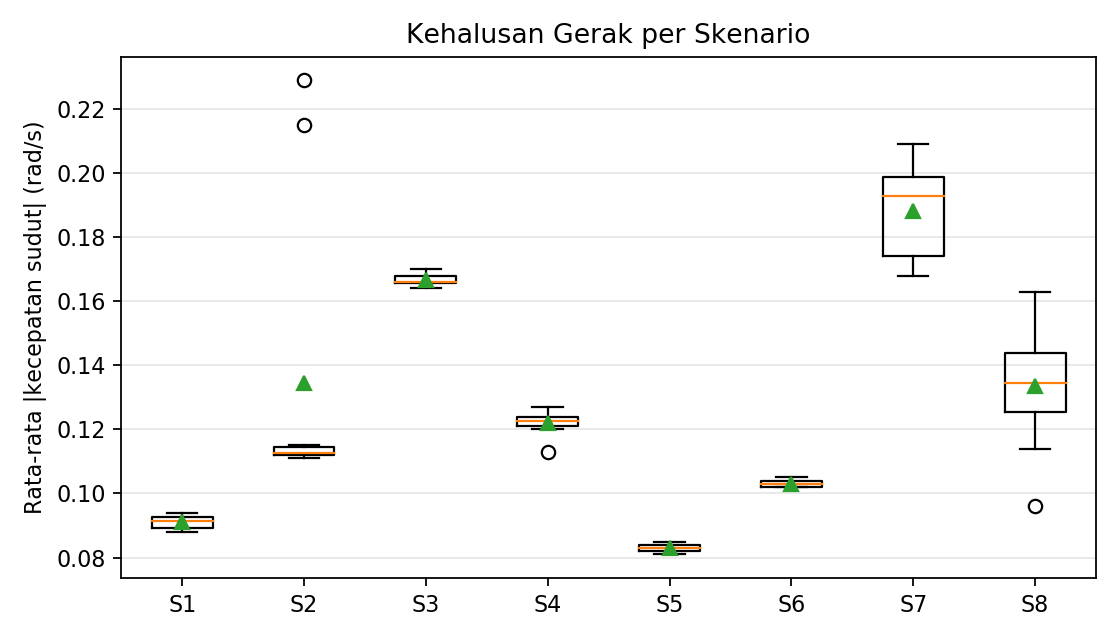
\includegraphics[width=0.75\textwidth]{gambar/fig_smoothness_box.png}
\caption{Distribusi rata-rata kecepatan angular pada seluruh skenario pengujian.}
\label{fig:smoothness_boxplot}
\end{figure}

Secara umum terlihat bahwa nilai kecepatan angular meningkat seiring bertambahnya kompleksitas lingkungan. Pada skenario tanpa obstacle, robot bergerak relatif lurus menuju tujuan sehingga hanya memerlukan sedikit koreksi arah. Ketika obstacle mulai muncul pada jalur navigasi, robot harus melakukan manuver penghindaran yang menyebabkan peningkatan kecepatan angular.

Perbedaan yang lebih jelas terlihat pada pasangan skenario yang melibatkan obstacle berp\-rofil rendah dan obstacle dinamis. Pada konfigurasi baseline, robot cenderung melakukan perubahan arah yang lebih mendadak ketika obstacle berada pada jarak yang dekat. Kondisi tersebut menyebabkan variasi kecepatan angular yang lebih besar selama navigasi berlangsung.

Sebaliknya, konfigurasi fuzzy menunjukkan distribusi kecepatan angular yang lebih terkendali. Meskipun robot melakukan manuver penghindaran yang lebih awal dan mempertahankan jarak aman yang lebih besar terhadap obstacle, perubahan orientasi yang terjadi cenderung lebih bertahap. Hal ini menunjukkan bahwa pengendali fuzzy mampu menghasilkan respons navigasi yang lebih halus dibandingkan konfigurasi baseline.

\subsection{Pengaruh Fuzzy terhadap Kehalusan Navigasi}

Peningkatan kehalusan pergerakan pada konfigurasi fuzzy berkaitan langsung dengan me\-kanisme adaptasi parameter yang diterapkan pada APFPlanner. Ketika obstacle terdeteksi pada jarak dekat atau nilai traversability lingkungan menurun, sistem fuzzy tidak hanya meningkatk\-an penguatan gaya tolak (\textit{repulsive gain}), tetapi juga menurunkan skala kecepatan robot secara bertahap.

Pendekatan tersebut menyebabkan robot mulai melakukan manuver penghindaran sebelum memasuki kondisi yang berisiko tinggi. Akibatnya, perubahan arah yang dilakukan menjadi lebih gradual dibandingkan konfigurasi baseline yang menggunakan parameter tetap. Dengan kata lain, robot tidak perlu melakukan koreksi arah yang agresif karena proses penghindaran obstacle telah dimulai lebih awal.

Karakteristik tersebut juga konsisten dengan hasil yang diperoleh pada Subbab~4.4 dan Subbab~4.5. Peningkatan \textit{minimum clearance} menunjukkan bahwa robot mempertahankan jarak aman yang lebih besar terhadap obstacle, sedangkan peningkatan waktu tempuh menunjukkan bahwa robot bergerak lebih konservatif. Kedua efek tersebut berkontribusi terhadap terbentuknya pola navigasi yang lebih stabil dan lebih halus selama perjalanan menuju tujuan.

\subsection{Implikasi terhadap Stabilitas Sistem Navigasi}

Dari sudut pandang navigasi robot bergerak, pergerakan yang lebih halus memiliki beberapa keuntungan. Pertama, osilasi yang lebih kecil mengurangi kemungkinan robot memasuki kondisi lokal yang tidak stabil ketika berinteraksi dengan obstacle. Kedua, perubahan arah yang lebih gradual menghasilkan lintasan yang lebih mudah diprediksi. Ketiga, perilaku navigasi yang lebih stabil berpotensi meningkatkan kenyamanan dan keamanan apabila sistem diterapkan pada lingkungan yang melibatkan interaksi dengan manusia.

Hasil pengujian menunjukkan bahwa integrasi kamera termal dan pengendali fuzzy tidak hanya meningkatkan keselamatan navigasi melalui peningkatan \textit{minimum clearance}, tetapi juga menghasilkan perilaku navigasi yang lebih stabil. Dengan demikian, manfaat metode yang diusulkan tidak terbatas pada kemampuan menghindari obstacle, tetapi juga mencakup peningkatan kualitas pergerakan robot secara keseluruhan.


\section{Evaluasi Deteksi Obstacle pada Area Blind-Spot LiDAR}
\label{sec:blindspot}
Salah satu tujuan utama penelitian ini adalah mengatasi keterbatasan LiDAR 2D dalam mendeteksi obstacle yang berada di luar bidang pindai horizontal sensor. Sebagaimana dijelaskan pada Bab~I dan Bab~III, LiDAR 2D hanya melakukan pengukuran pada satu bidang datar sehingga obstacle yang memiliki tinggi lebih rendah dari bidang pemindaian berpotensi tidak terdeteksi meskipun secara fisik berada pada jalur pergerakan robot (\cite{Fagundes2024,Kibii2022}). Kondisi tersebut dikenal sebagai \textit{blind-spot} vertikal dan menjadi salah satu penyebab utama terjadinya kolisi pada sistem navigasi yang hanya mengandalkan sensor LiDAR 2D.

Untuk mengevaluasi kemampuan sistem dalam mengatasi permasalahan tersebut, pada penelitian ini digunakan obstacle berprofil rendah berupa model kucing yang ditempatkan pada jalur navigasi robot. Obstacle tersebut dirancang agar sebagian besar berada di luar bidang observasi LiDAR sehingga tidak dapat direpresentasikan secara memadai pada data \textit{LaserScan}. Sebaliknya, obstacle masih dapat diamati oleh kamera termal sehingga informasi keberadaannya dapat dimanfaatkan dalam proses pembentukan traversability termal dan \textit{virtual scan}.

\subsection{Perbandingan Kejadian Tabrakan pada Obstacle Blind-Spot}

Jumlah kejadian tabrakan terhadap obstacle kucing pada seluruh skenario yang mengandung area \textit{blind-spot} ditunjukkan pada Gambar~\ref{fig:cat_collision}.

\begin{figure}[H]
\centering
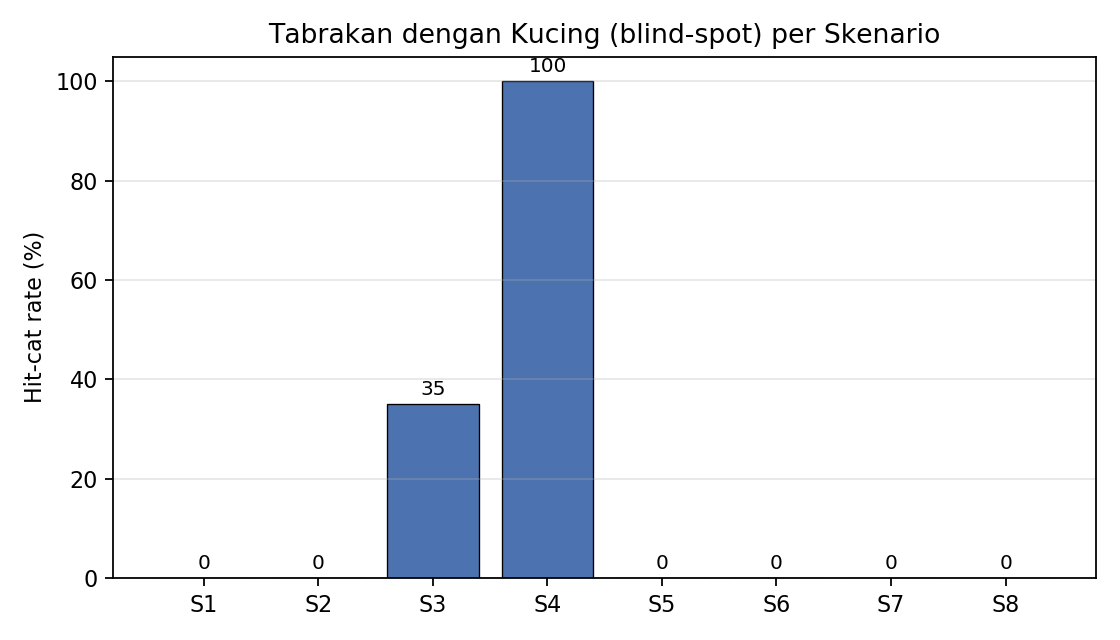
\includegraphics[width=0.75\textwidth]{gambar/fig_hit_cat.png}
\caption{Jumlah kejadian tabrakan terhadap obstacle berprofil rendah pada area blind-spot LiDAR.}
\label{fig:cat_collision}
\end{figure}

Hasil pengujian menunjukkan bahwa konfigurasi baseline mengalami kegagalan yang leb\-ih sering ketika berhadapan dengan obstacle berprofil rendah. Pada konfigurasi ini, sebagian obstacle tidak terdeteksi secara memadai oleh LiDAR sehingga robot tetap bergerak menuju tujuan tanpa melakukan manuver penghindaran yang cukup.

Sebaliknya, konfigurasi fuzzy yang memanfaatkan integrasi kamera termal menunjukkan penurunan jumlah kejadian tabrakan yang sangat signifikan. Informasi termal yang diperoleh dari kamera memungkinkan sistem mengenali keberadaan obstacle meskipun obstacle tersebut berada di luar bidang pemindaian LiDAR. Informasi tersebut kemudian diproyeksikan ke dalam representasi navigasi melalui proses pembentukan \textit{virtual scan} dan perhitungan traversability sehingga obstacle dapat diperhitungkan oleh planner lokal selama proses navigasi.

Temuan ini konsisten dengan hasil pada Subbab~4.3 dan Subbab~4.4 yang menunjukkan peningkatan \textit{Success Rate}, \textit{Collision-Free Rate}, dan \textit{minimum clearance} pada konfigurasi fuzzy. Dengan kata lain, peningkatan performa yang diamati tidak hanya berasal dari perubahan strate\-gi navigasi, tetapi juga dari peningkatan kualitas persepsi lingkungan yang diperoleh melalui integrasi kamera termal.

\subsection{Kontribusi Kamera Termal terhadap Persepsi Lingkungan}

Keunggulan utama kamera termal pada penelitian ini terletak pada kemampuannya menyediakan informasi tambahan pada area yang tidak dapat diamati secara optimal oleh LiDAR 2D. Ketika obstacle berada di luar bidang pemindaian laser, data LiDAR tidak lagi cukup untuk merepresentasikan kondisi lingkungan secara lengkap. Pada kondisi tersebut, kamera termal berperan sebagai sensor komplementer yang menyediakan informasi keberadaan obstacle berdasarkan karakteristik termalnya.

Berbeda dengan pendekatan yang hanya menggunakan kamera sebagai sensor deteksi objek, penelitian ini memanfaatkan informasi termal untuk membentuk estimasi traversability lingkungan yang kemudian digabungkan dengan traversability berbasis LiDAR melalui meka\-nisme fusi sensor. Pendekatan tersebut memungkinkan sistem menghasilkan representasi lingk\-ungan yang lebih lengkap tanpa mengubah struktur dasar ROS Navigation Stack yang digunakan.

Hasil eksperimen menunjukkan bahwa kombinasi antara traversability LiDAR, traversability termal, dan pengendali fuzzy menghasilkan peningkatan kemampuan navigasi terutama pada kondisi yang sebelumnya menjadi kelemahan utama LiDAR 2D. Dengan demikian, kamera termal tidak hanya berfungsi sebagai sensor tambahan, tetapi berperan langsung dalam meningkatkan keselamatan navigasi melalui pengurangan risiko tabrakan terhadap obstacle pada area \textit{blind-spot}.

\subsection{Implikasi terhadap Tujuan Penelitian}

Berdasarkan seluruh hasil pengujian yang telah dipaparkan pada Subbab~4.3 hingga Subbab~4.7, dapat disimpulkan bahwa metode yang diusulkan berhasil mengatasi sebagian keterbatasan persepsi yang dimiliki LiDAR 2D pada lingkungan indoor. Integrasi kamera termal memungkinkan obstacle berprofil rendah tetap terdeteksi meskipun tidak berada pada bidang pemindaian laser, sedangkan mekanisme fuzzy membantu robot merespons kondisi tersebut secara adaptif melalui penyesuaian parameter navigasi.

Temuan ini mendukung hipotesis bahwa fusi sensor LiDAR dan kamera termal mampu meningkatkan keselamatan navigasi robot bergerak pada lingkungan yang mengandung obstacle berprofil rendah. Selain meningkatkan \textit{minimum clearance}, metode yang diusulkan juga mempertahankan tingkat keberhasilan navigasi yang tinggi serta mengurangi kejadian tabrakan pada area yang sebelumnya menjadi \textit{blind-spot} bagi LiDAR 2D.

